\section{Three-dimensional disks with beta cooling}\label{3ddisk}
We now extend the previous results to 3D disks with vertical
structure. This is expected to weaken gravitational instabilities by
`diluting' self-gravity along the vertical direction. It is possible to incorportate
this effect in the previous 2D framework, but this introduces
additional parameters. We discuss this in Appendix \ref{3dcorr}. 
It is more direct to solve the 3D eigenvalue problem to avoid such 
uncertainties.  

{\bf note: fast beta-cooling in 3D destablizes vertical modes (enables
convection)}

%take k>0 wlog
%consider Gamma=1
%height s.t. rho(zmax) = 0.05 rho(0) avoid very low densities 
\subsection{Numerical procedure}
We use a pseudo-spectral method to solve the set of ordinary
differential equations, Eq. \ref{lin_mass}---\ref{lin_gravity}, on 
the domain $ z\in[0,\zmax]$ with a parity condition at the midplane.
We expand $\bm{U}=[\delta P,\delta\rho,\delta\Phi,
  \delta v_x, \delta 
  v_y]$ in even Chebyshev polynomials,
\begin{align}
  \bm{U}(z) = \sum_{j=1}^N \bm{a}_jT_{2(j-1)}(z/\zmax), 
\end{align}
and the vertical velocity in odd Chebyshev polynomials,
\begin{align}
  \delta v_z(z) = \sum_{j=1}^N b_jT_{2j-1}(z/\zmax),   
\end{align}
where $\bm{a}_j$ and $b_j$ are the spectral coefficients. 
The basis functions are chosen to satisfy a reflecting boundary
condition at the midplane, %GI has even symmetry across midplane 
\begin{align}
  \bm{U}^\prime(0) = \bm{0}, \quad \delta v_z(0) = 0.
\end{align}
%At the upper disk boundary we also apply reflection,
We explicitly apply a reflecting upper disk boundary, 
\begin{align}
  \delta v_z(\zmax) = \delta v_x^\prime(\zmax) = \delta
  v_y^\prime(\zmax) = 0,
\end{align}
and the potential satisfies
\begin{align}
  \delta \Phi^\prime (\zmax) + k \delta\Phi(\zmax) = 0, 
\end{align}
as derived by \cite{goldreich65a} and used in similar studies  
\citep{kim12,lin14c}. %reflection is standard in direct simulations 

We discretize the equations, including upper disk boundary conditions,
over the $N$ positive abscissae of the extrema of $T_{2N-1}$. This
procedure converts the differential equations into a generalized
eigenvalue problem, for which we use the standard matrix package
LAPACK to solve.  

In the following examples we consider a vertically isothermal disk
($\Gamma=1$) with a numerical surface such 
that $\rho(\zmax)=0.05\rho_0$, and use $N=65$. 

%in practice eliminate density with poisson
\subsection{Inviscid disk}

Fig. \ref{3d_inviscid} show growth rates and the most unstable wavenumber
obtained for a 3D inviscid disk without irradiation. We also plot 2D
results with the 3D correction as described in Appendix
\ref{3dcorr}. While the chosen value of $H_\mathrm{sg}$ results in a close
match between 2D and 3D growth rates, the 3D wavenumber is somewhat
smaller. This reflects self-gravity being weakened in the verical
direction: a larger horizontal scale is required to achieve the same
strength of self-gravity (and hence growth rate) as the 2D case.  

\begin{figure}
  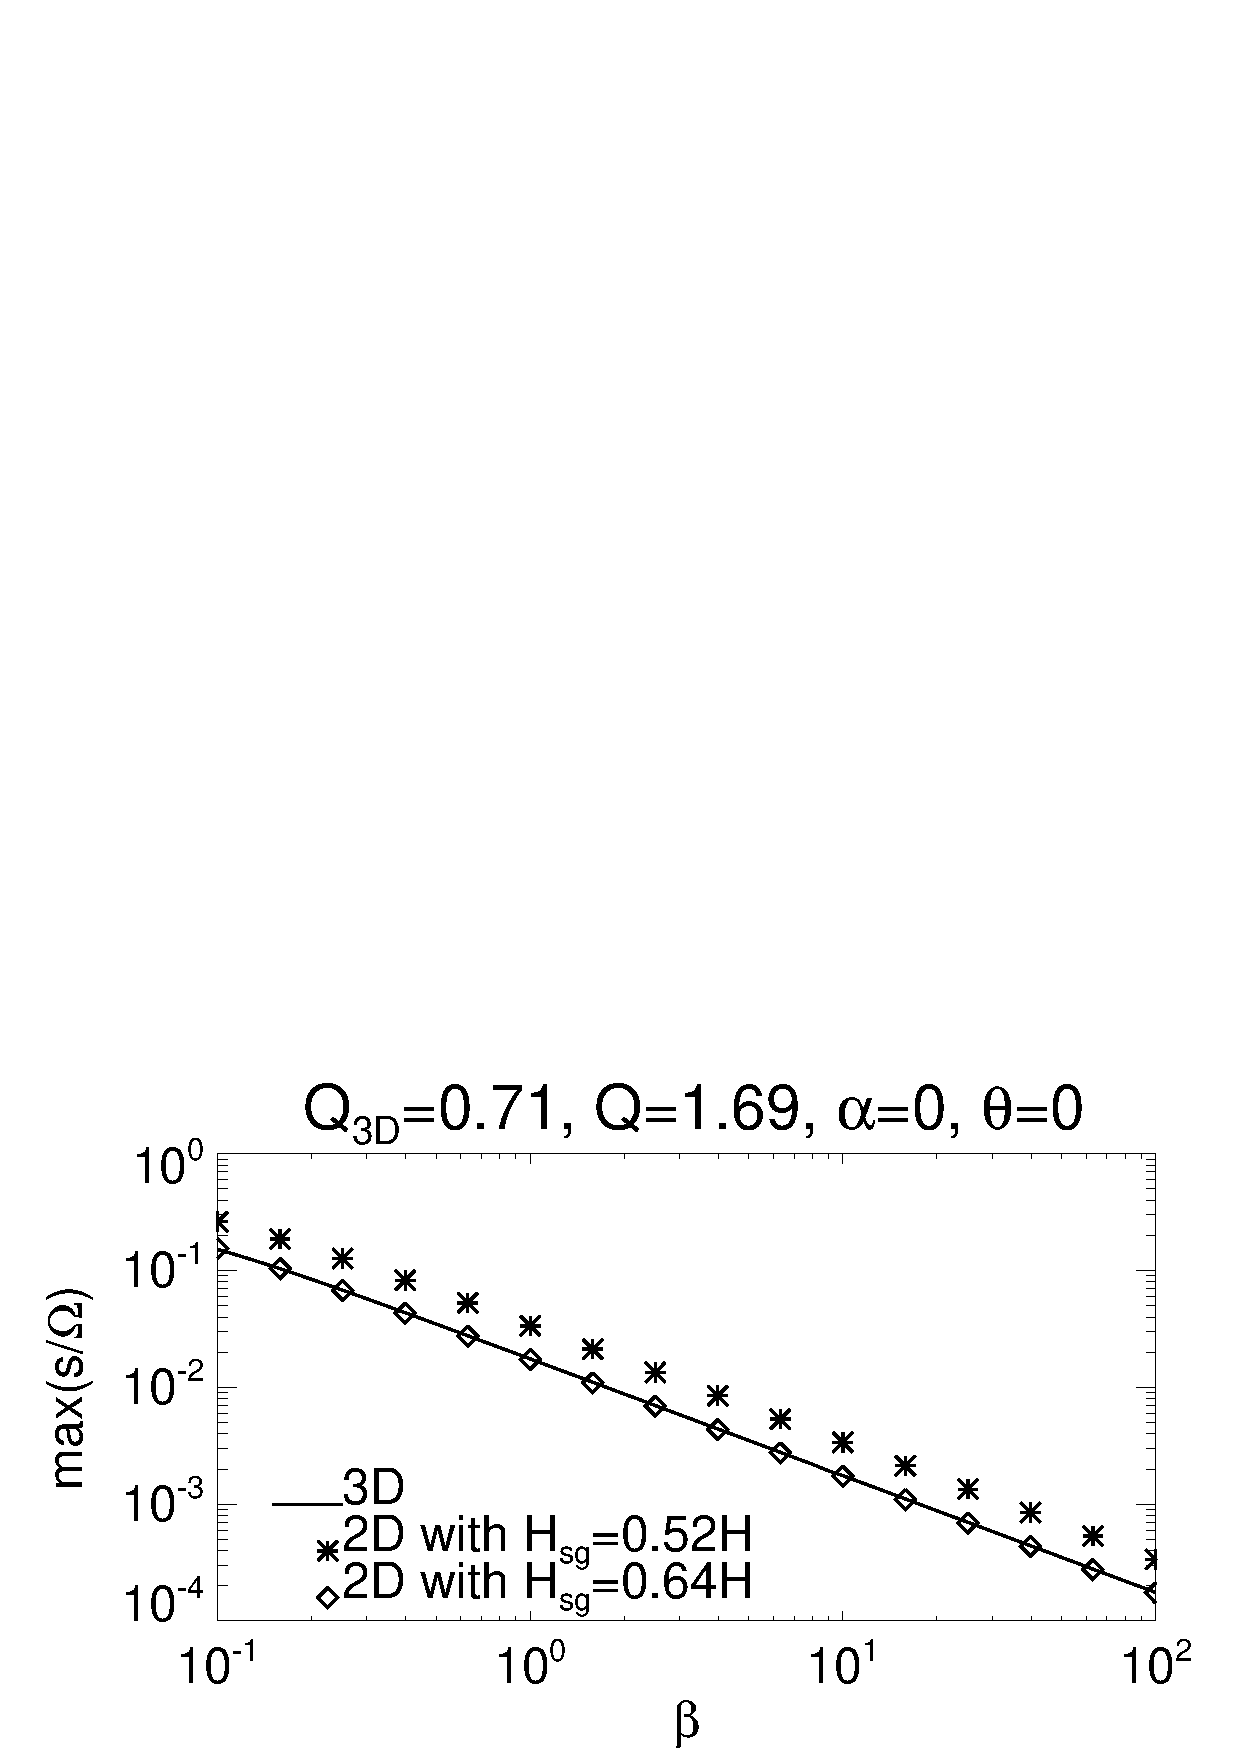
\includegraphics[width=\linewidth,clip=true,trim=0cm 1.5cm 0.23cm
    0.0cm]{figures/3d_inviscid_rates}\\
  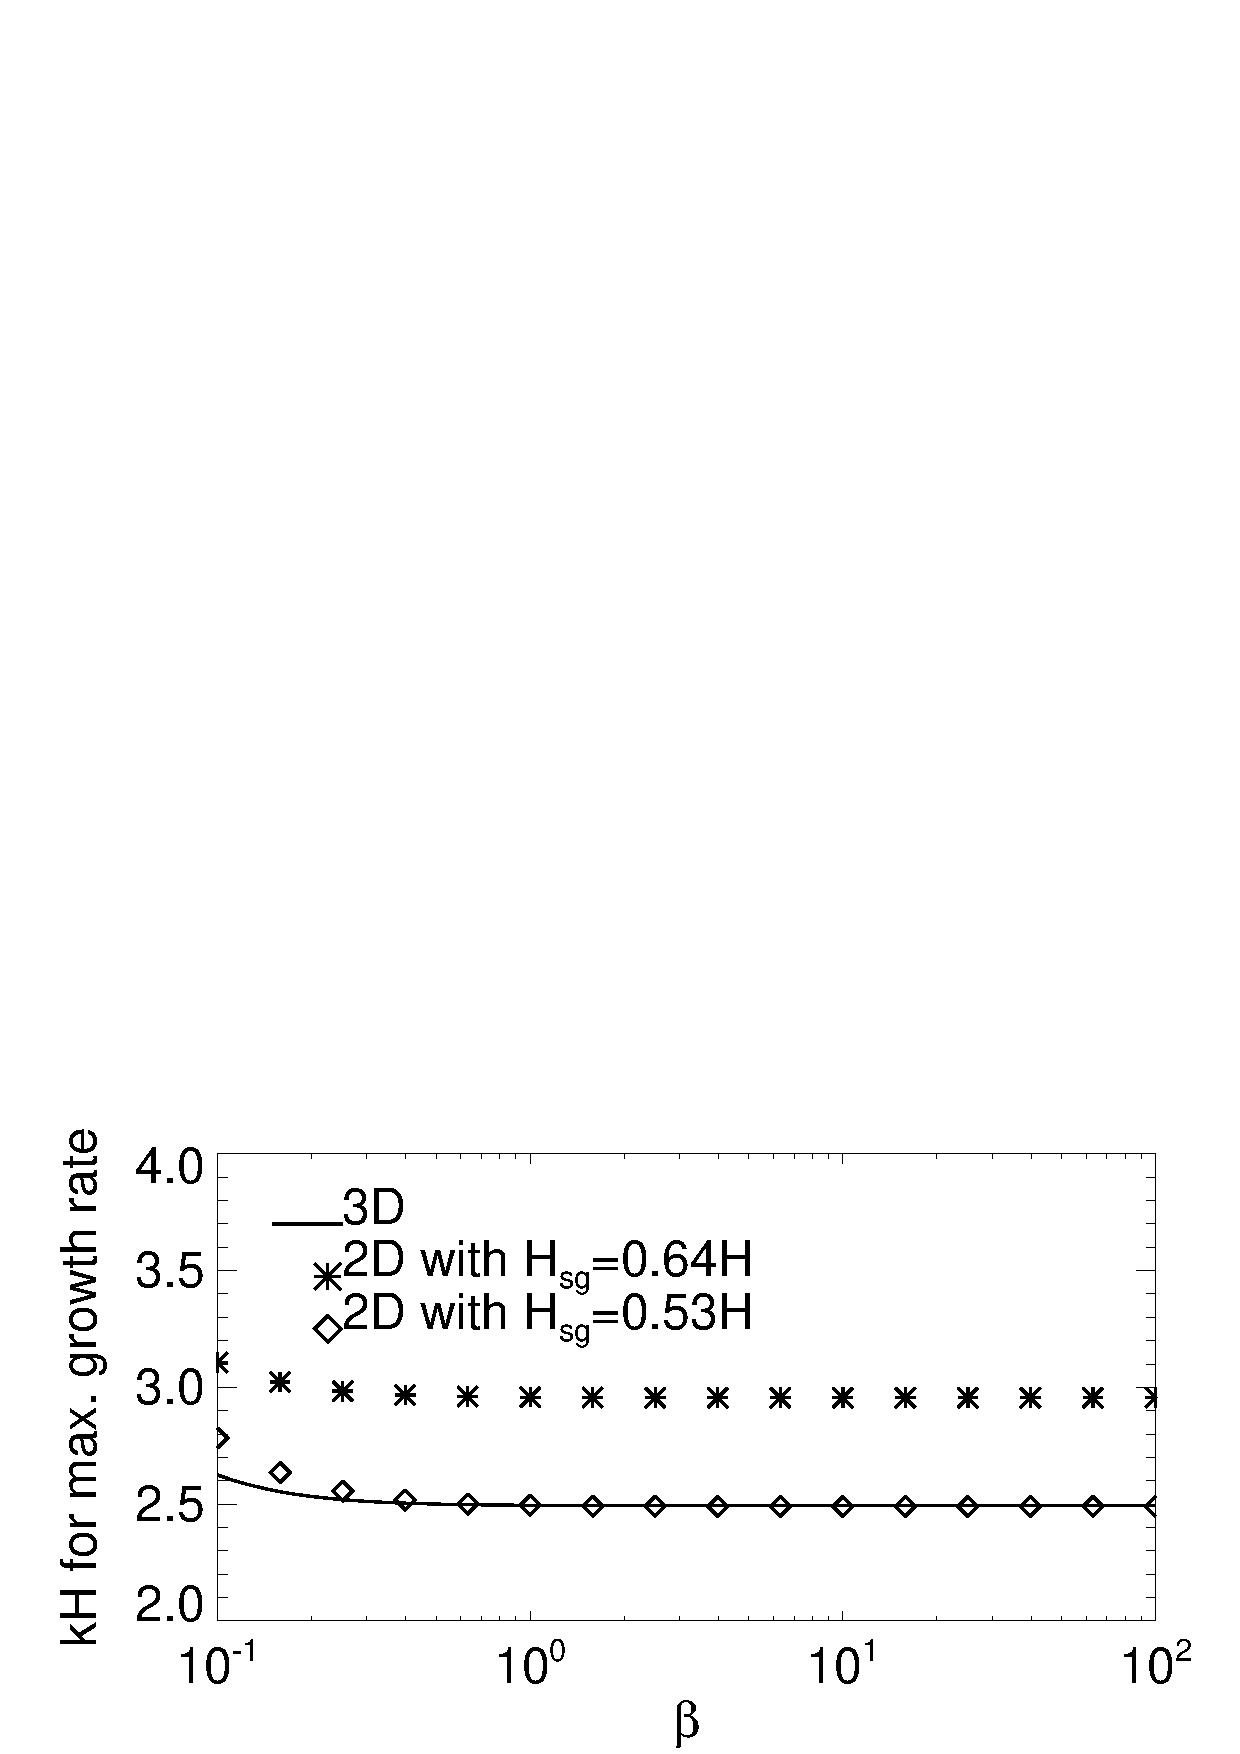
\includegraphics[width=\linewidth,clip=true,trim=0cm 0cm 0.23cm
    0.88cm]{figures/3d_inviscid_kmax}
  \caption{Growth rates (top) and optimal wavenumber (bottom) obtained
    from the 3D eigenvalue problem (solid line). Asterisks are
    corresponding values from the 2D dispersion relation
    (Eq. \ref{thindisk}) but with a modified gravitational constant
    as described in Appendix \ref{3dcorr}. \label{3d_inviscid}}
\end{figure}

\subsection{Viscous disk} %growth rates, kmax, eigenfunction
For the 3D viscous problem we use the same set up as that in 2D
(\S\ref{2dvisc}), but with 
\begin{align*}
  \qvert = \frac{Q_\mathrm{3D,crit}}{\sqrt{\alpha}}, 
\end{align*}
where $Q_\mathrm{3D,crit}\simeq0.36$ is the 3D equivalent to the 2D
critical value, $Q_\mathrm{crit}$. 

Fig. \ref{3d_visc} show growth rates, maximized over $k$, as a
function of the cooling time $\beta$. We also plot 2D results with 3D
corrections. Softening the self-gravity in 2D captures the correct 
qualitative behavior as in the full 3D case, but it is clear that a
single, constant value of $H_\mathrm{sg}$ cannot re-produce 3D growth 
rates for all $\beta$. 
This suggests that the exact value of
$H_\mathrm{sg}$ is problem-dependent (cooling and viscosity), although taking
$H_\mathrm{sg}\sim O(H)$ should give the correct 3D growth rate within
a factor of two. In this respect it is easier to
directly solve the 3D problem.  

\begin{figure}
  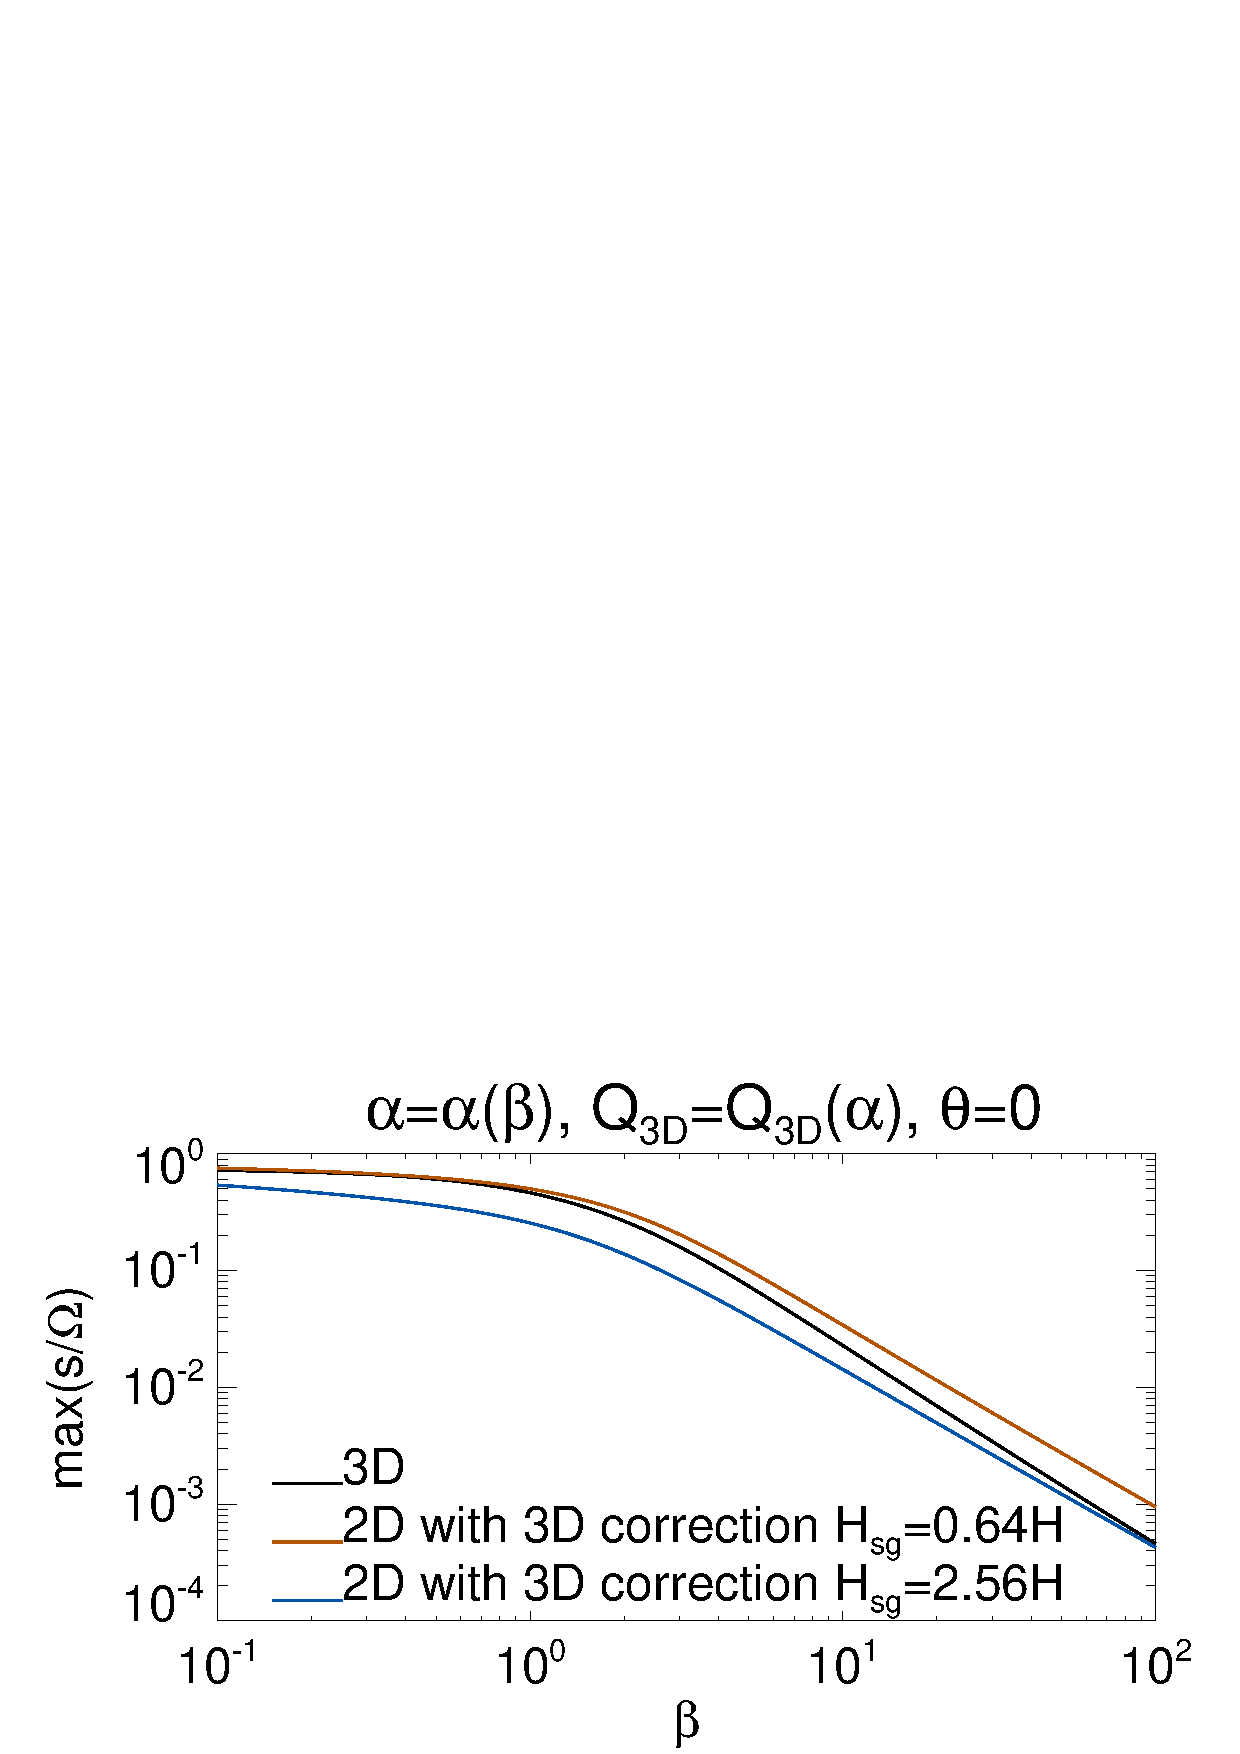
\includegraphics[width=\linewidth,clip=true,trim=0cm 0.cm 0.23cm
    0.0cm]{figures/growth_visc3d}
  \caption{Growth rates from the viscous 3D eigenvalue problem (black solid
    line). The other curves are obtained from the 2D dispersion
    relation (Eq. \ref{thindisk}) but with a modified gravitational
    constant as described in Appendix \ref{3dcorr}. \label{3d_visc}}
\end{figure}
